%b Reconstructed dynamics of variation in chromatin accessibility profiles across the developmental trajectory. Shown are profiles of representative cells for Rock2 and Efhd1. Axis ticks display –200 bp, 0 bp and +200 bp relative to the TSS. Shading is used to highlight changes between cells. c Developmental trajectory is associated changes in genome-wide methylation-accessibility coupling. Shown is the location of each cell in pseudotime (x axis) and the corresponding Pearson correlation coefficients between methylation and accessibility (y axis) in different genomic contexts

% (EXPLAIN BETTER..) Next, we aimed at identifying genes with coordinated promoter accessibility changes along the trajectory. To do this, we quantified for each gene the Spearman's rank coefficient between the cell's non-linear chromatin accessiiblity profile and the corresponding position in the pseudotime. This identified 15 significant genes, most of them showing a positive coefficient linked to a decrease in chromatin accessibility along the trajectory.

% \begin{figure}[H]
% 	\centering
% 	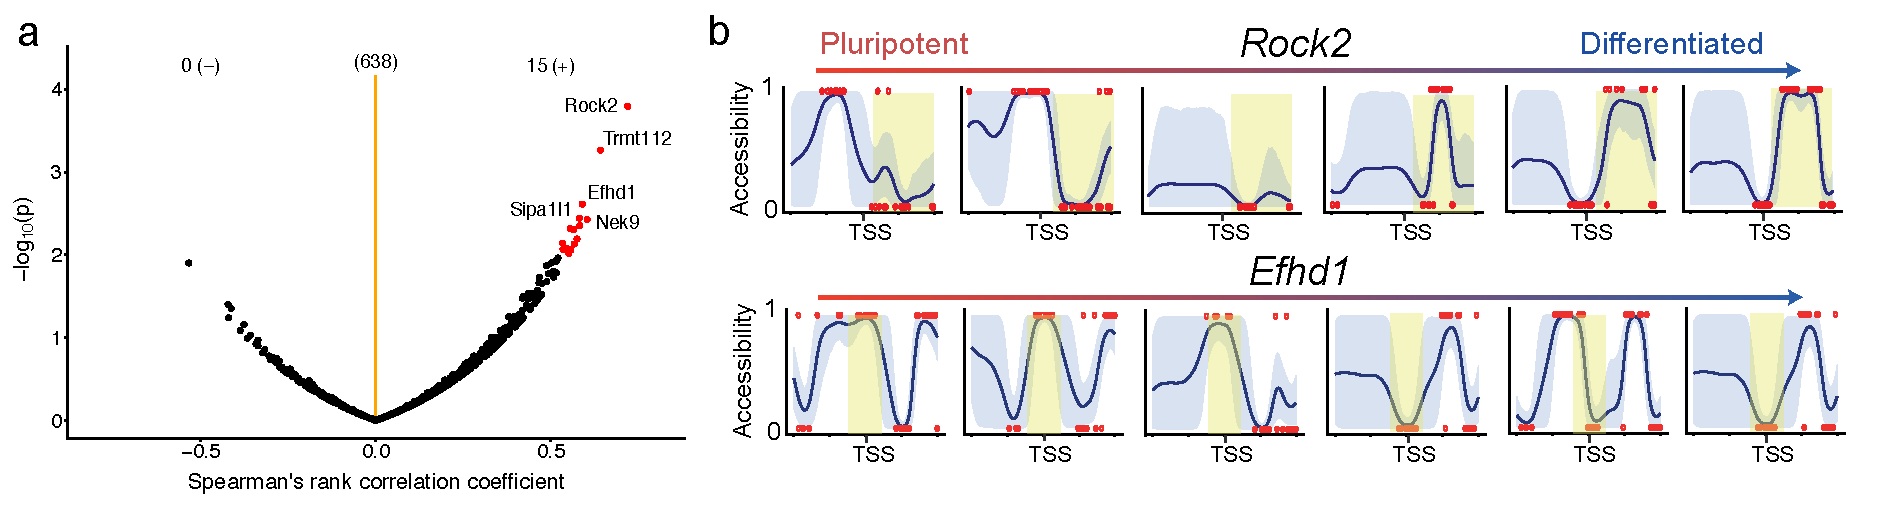
\includegraphics[width=0.9\linewidth]{scNMT_pseudotime_correlation}
% 	\caption[]{}
% 	\label{fig:scnmt_pseudotime_correlation}
% \end{figure}

% Association analysis between promoter accessibility profile and development trajectory. For each gene, the cell cluster assignments were associated with the corresponding cell’s position in the pseudotime axis using Spearman’s rank coefficient. Shown is a volcano plot of correlation coefficients in the x axis with the corresponding log10 p-values in the y axis. Red dots denote genes that pass statistical significance threshold (alpha = 0.01).
% Reconstructed dynamics of chromatin accessibility profiles along the developmental trajectory. Shown are profiles of representative cells for genes that show dynamic behaviour along the pseudotime in their accessibility profile: (a) Nek9 and (b) Trmt112. Each red dot represents a GpC site, with binary accessibility value (1=accessible, 0=inaccessible). A non-linear regression curve is fit for each gene and cell using the BPRMeth package5. The blue line represents the mean of the posterior distribution of the inferred non- linear function, and the shading represents the corresponding 80% credible interval. Axis ticks display windows of +-200bp around the TSS. Yellow shading is used to highlight the relevant region of dynamic changes.